%================================================================
\section{Methodology}\label{sec:Method}
%================================================================

%----------------------------------------------------------------
\subsection{Data processing}
%----------------------------------------------------------------
\subsubsection{The MNIST dataset}


The original MNIST dataset consists of 60,000 training and 10,000 test images of 28x28 pixel grayscale images of handwritten digits (0-9). Each image is labeled with the corresponding digit. The pixel values in the original dataset range from 0 to 255, representing the intensity of grayscale. In our experiments, we reduce the complexity of the dataset by binarizing the images. All pixel values greater than or equal to 127 are set to 1 (white), while values below 127 are set to 0 (black). The binarized MNIST dataset is commonly used in machine learning tasks where feature extraction is based on the presence or absence of pixels rather than the grayscale intensity.

In order to speed up training for our experiments, we only train and test the model on images with the labels 0-3. Samples from the training set are shown in \autoref{fig:bmnist}.

\begin{figure}[!htb]
\begin{center}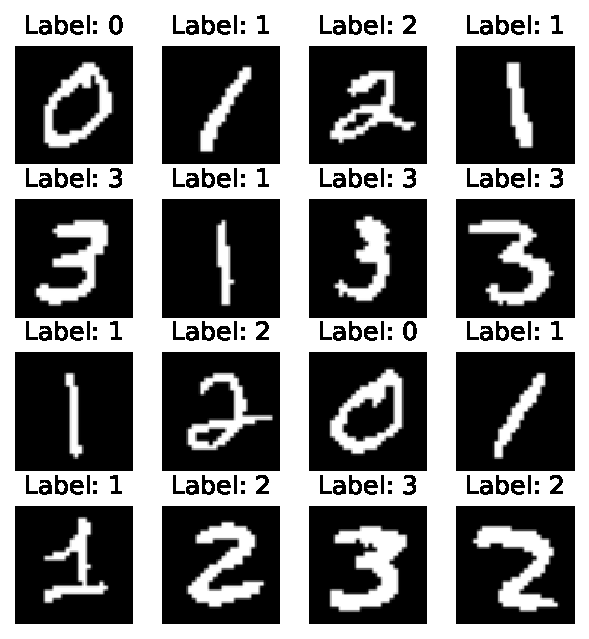
\includegraphics[scale=0.7]{latex/figures/bmnist.pdf}
\end{center}
\caption{Samples from the binarized MNIST dataset with labels 0-3.}
\label{fig:bmnist}
\end{figure}


%----------------------------------------------------------------
\subsection{Models}
%----------------------------------------------------------------
\subsubsection{MLP-VAE}

\subsubsection{DNN-VAE}

\subsubsection{Conv-VAE}

\url{https://www.tensorflow.org/tutorials/generative/cvae}

\subsection{Activation function and weight initialization}

ReLU, He init

%----------------------------------------------------------------
\subsection{Training}
%----------------------------------------------------------------

\subsubsection{The NAdamW optimizer}


Adam with weight decay regularization.

AdamW uses weight decay to regularize learning towards small weights, as this leads to better generalization. In SGD you can also use L2 regularization to implement this as an additive loss term, however L2 regularization does not behave as intended for adaptive gradient algorithms such as Adam, see [Loshchilov et al, 2019].

Let $\alpha_t$ represent the learning rate and $\beta_1, \beta_2$,
$\varepsilon$, $\bar{\varepsilon}$  represent the arguments
b1, b2, eps and eps\_root respectively. The learning rate is
indexed by $t$ since the learning rate may also be provided by a
schedule function. Let $\lambda$ be the weight decay and 
$\theta_t$ the parameter vector at time $t$.

The init function of this optimizer initializes an internal state
$S_0 := (m_0, v_0) = (0, 0)$, representing initial estimates for the
first and second moments. In practice these values are stored as pytrees containing all zeros, with the same shape as the model updates.
At step $t$, the update function of this optimizer takes as
arguments the incoming gradients :$g_t$, the optimizer state $S_t$ 
and the parameters $\theta_t$ and computes updates $u_t$ and 
new state $S_{t+1}$. Thus, for $t > 0$, we have,

\begin{align*}
  m_t &\leftarrow \beta_1 \cdot m_{t-1} + (1-\beta_1) \cdot g_t \\
  v_t &\leftarrow \beta_2 \cdot v_{t-1} + (1-\beta_2) \cdot {g_t}^2 \\
  \hat{m}_t &\leftarrow m_t / {(1-\beta_1^t)} \\
  \hat{v}_t &\leftarrow v_t / {(1-\beta_2^t)} \\
  u_t &\leftarrow -\alpha_t \cdot \left( \hat{m}_t / \left({\sqrt{\hat{v}_t 
  + \bar{\varepsilon}} + \varepsilon} \right) + \lambda \theta_{t} \right)\\
  S_t &\leftarrow (m_t, v_t).
\end{align*}

This implementation can incorporate a momentum a la Nesterov introduced by [Dozat 2016]. The resulting optimizer is then often referred as NAdamW. With the keyword argument `nesterov=True`, the optimizer uses Nesterov momentum, replacing the above $\hat{m}_t$ with

 \begin{equation*}
    \hat{m}_t \leftarrow
    \beta_1 m_t / {(1-\beta_1^{t+1})} + (1 - \beta_1) g_t / {(1-\beta_1^t)}. 
 \end{equation*}


\subsubsection{Learning rate scheduler}

The learning rate is one of the most important hyperparameters for training deep neural networks, as it determines the size of the steps taken during the optimization process. Instead of employing a fixed learning rate, it is common to dynamically adjust the learning rate during training according to a schedule. A learning rate scheduler can notably enhance convergence and overall model performance. In the training of the VAEs, we will use the \textit{cosine decay schedule} \citep{cosine_decay}. It starts with an initial learning rate and gradually decreases the learning rate following a cosine curve. The learning rate at iteration $t$ is given by

\begin{equation}\label{eq:cosine_decay}
    \frac{I \qty(1 - \alpha)}{2} \qty(1 + \cos \qty(\pi \frac{t}{T})^p) + \alpha,
\end{equation}

where $T$ is the number of decay steps, $p$ is an exponent that can be used to modify the decay curve, $I$ is the initial learning rate and $\alpha$ determines the final learning rate as a fraction of the initial learning rate. During training, we set 
\begin{align*}
    T &= \text{number of examples in a batch} \times \text{number of epochs}, \\
    p &= 1, \\
    I &= 10^{-3}, \\
    \intertext{and}
    \alpha &= 10^{-2}
\end{align*}
which means that the final learning rate will be $10^{-5}$. \autoref{fig:lr_schedule} illustrates the cosine decay scheduler.

\begin{figure}[!htb]
\begin{center}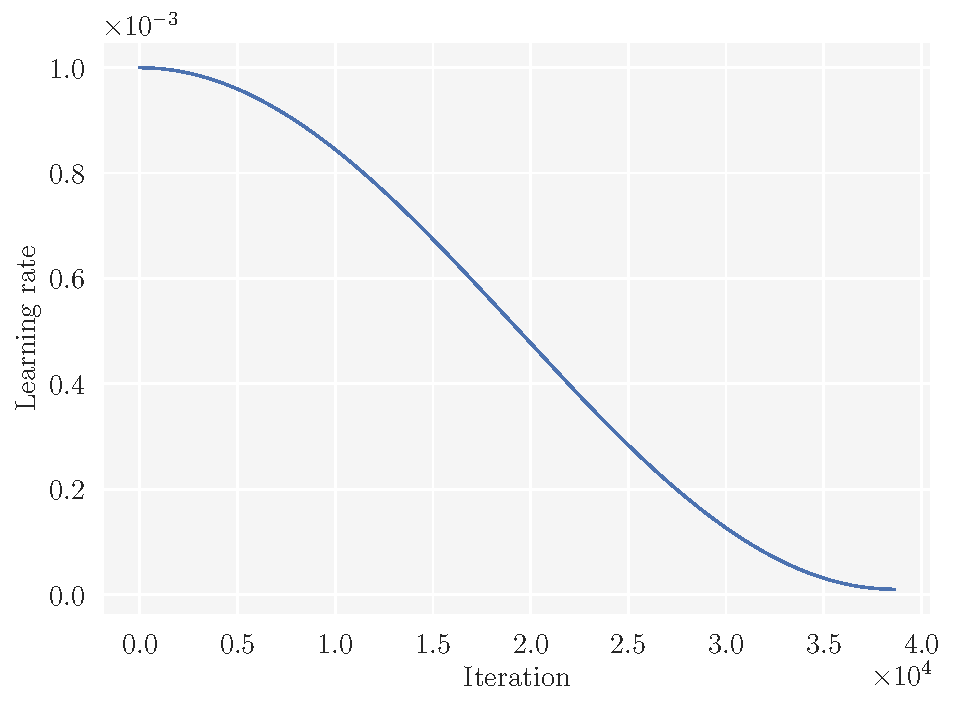
\includegraphics[scale=0.7]{latex/figures/lr_schedule.pdf}
\end{center}
\caption{Illustration of the cosine decay learning rate scheduler given by \autoref{eq:cosine_decay}. The variables of the cosine decay scheduler are set according to the description in the main text with 386 examples in one batch and 50 epochs.}
\label{fig:lr_schedule}
\end{figure}


\subsubsection{Loss functions}

\url{https://storage.googleapis.com/deepmind-media/UCLxDeepMind_2020/L11%20-%20UCLxDeepMind%20DL2020.pdf}

\url{https://www.expunctis.com/2019/01/27/Loss-functions.html}

\url{https://machine-learning-note.readthedocs.io/en/latest/basic/loss_functions.html}



